% \documentclass[12pt, twoside]{article}
\usepackage[letterpaper, margin=1in, headsep=0.2in]{geometry}
\setlength{\headheight}{0.6in}
%\usepackage[english]{babel}
\usepackage[utf8]{inputenc}
\usepackage{microtype}
\usepackage{amsmath}
\usepackage{amssymb}
%\usepackage{amsfonts}
\usepackage[nomessages]{fp} %\FPeval{\var-name}{2*sin(pi/6)}
\usepackage{siunitx} %units in math. eg 20\milli\meter
\usepackage{yhmath} % for arcs, overparenth command
\usepackage{tikz} %graphics
\usetikzlibrary{quotes, angles, arrows, arrows.meta}
\usepackage{graphicx} %consider setting \graphicspath{{images/}}
\usepackage{parskip} %no paragraph indent
\usepackage{enumitem}
\usepackage{multicol}
\usepackage{venndiagram}

\usepackage{fancyhdr}
\pagestyle{fancy}
\fancyhf{}
\renewcommand{\headrulewidth}{0pt} % disable the underline of the header
\raggedbottom
\hfuzz=2mm %suppresses overfull box warnings

\usepackage{hyperref}

\fancyhead[LE]{\thepage}
\fancyhead[RO]{\thepage \\ Name: \hspace{4cm} \,\\}
\fancyhead[LO]{BECA / Dr. Huson / Geometry\\*  Unit 1: Segments, length, and area\\* 20 Sept 2022}

\begin{document}

\subsubsection*{1.8 Homework: Area of rectangles, triangles, parallelograms}
\begin{enumerate}
\item Find the area of $\triangle ABC$. The altitude $h$ of the triangle is $8$ centimeters and the base $AB=10 \frac{1}{2}$ cm. (diagram not to scale) \par
  \begin{tikzpicture}[scale=1]
    \draw[thick]
      (0,0)node[below]{$A$}--
      (6,0)node[below]{$B$}--
      (4,3)node[above]{$C$}--cycle;
   \draw[dashed] (4,0)--(4,3);
   \draw (4,0)++(0.3,0)--++(0,0.3)--+(-0.3,0);
   \node at (3.3,1.2){$h=8$};
   \node at (3,0)[below]{$10 \frac{1}{2}$ cm};
  \end{tikzpicture}

\item Find the area $A$ and perimeter $P$ of the shape shown below. The grid is in centimeters.
  \begin{flushleft}
    \begin{tikzpicture}[scale=1]
      \draw[help lines] (-4,-4) grid (5,3);
      \draw[thick, -] (-3,-3)--(4,-3)--(4,2)--(2,2)--(2,0)--(-1,0)--(-1,2)--(-3,2)--cycle;
    \end{tikzpicture}
  \end{flushleft}

\item Find the length of the base of a rectangle with area $A=22 \frac{1}{2}$ and height $h=5$, expressed as a fraction. Start with the form (use $b$ or $x$): \par \medskip
$A = b \times h = 22 \frac{1}{2}$
  \begin{flushright}
  \begin{tikzpicture}[scale=1.25]
    \draw[thick] (0,0)--(3,0)--(3,3.5)--(0,3.5)--cycle;
    \node at (3.5, 2){5};
    \node at (1.5, -0.3){$?$};
    \node at (1.5, 2){$A = 22 \frac{1}{2}$};
  \end{tikzpicture}
  \end{flushright}

\newpage
\item The perimeter of a square is 40 centimeters. Find the length of the side of the square. \vspace{2cm}

\item Find the length of the base of a triangle with area $A=35$ and height $h=10$. Start with the form (use $b$ or $x$): \par \medskip
  $A = \frac{1}{2} \times b \times h = 35$
  \begin{flushright}
  \begin{tikzpicture}[scale=1.25]
    \draw[thick] (0,0)--(3,0)--(2.5,3.5)--cycle;
    \draw[<->,dashed] (3.3,0)--(3.3,3.5);
    \node at (3.6,1.7){10};
    \node at (1.5,0.3){$b=?$};
    \node at (1.8,1.4){$A = 35$};
  \end{tikzpicture}
  \end{flushright}


\item Find the area and perimeter of the combined rectangular shape shown below. Mark the missing side lengths first. \hfill \emph{(not drawn to scale)}
  \begin{flushleft}
  \begin{tikzpicture}[scale=1.3]
    \draw[thick] (2,0)--(4.5,0)--(4.5,2.5)--(3,2.5)--(3,5)--(2,5)--cycle;
    \node at (4.8, 1.2){6};
    \node at (3.9, 2.8){5};
    \node at (3.2, -0.3){7};
    \node at (1.6, 2.5){11};
  \end{tikzpicture}
  \end{flushleft} 

\item Rectangle $JKLM$ has area $A=21$ and base $JK=7$ but unknown height. Write an equation then solve. Start with this form (for the unknown, use $h$, $x$, or $KL$): \par \medskip
  $A = b \times h = 21$


\end{enumerate}
\end{document}